%%%%%%%%%%%%%%%%%%%%%%%%%%%%%%%%%%%%%%%%%%%%%%%%%%%%%%%%%%%%%%%%%%%%%%%%%%%%%%%%
%2345678901234567890123456789012345678901234567890123456789012345678901234567890
%        1         2         3         4         5         6         7         8


\documentclass[letterpaper, 10 pt, conference]{ieeeconf}  % Comment this line out
                                                          % if you need a4paper
%\documentclass[a4paper, 10pt, conference]{ieeeconf}      % Use this line for a4
                                                          % paper

\IEEEoverridecommandlockouts                              % This command is only
                                                          % needed if you want to
                                                          % use the \thanks command
\overrideIEEEmargins
% See the \addtolength command later in the file to balance the column lengths
% on the last page of the document

\usepackage{graphicx}
\usepackage{float}
\usepackage{graphics}
\usepackage[utf8]{inputenc}
%\usepackage[spanish, activeaccute]{babel} %permite escribir con ortografía en español, acentos, ñ, etc
\usepackage[spanish,es-noshorthands]{babel}
\usepackage{mathtools} %matematica
\usepackage{amsmath} %matematica
\usepackage{circuitikz} %pa dibujar circuitoz
\usepackage{siunitx} %simbologia, ohm etc
\usepackage{amssymb}


% Para los acentos
%\usepackage[spanish]{babel}
% The following packages can be found on http:\\www.ctan.org
%\usepackage{graphics} % for pdf, bitmapped graphics files
%\usepackage{epsfig} % for postscript graphics files
%\usepackage{mathptmx} % assumes new font selection scheme installed
%\usepackage{times} % assumes new font selection scheme installed
%\usepackage{amsmath} % assumes amsmath package installed
%\usepackage{amssymb}  % assumes amsmath package installed

\title{\LARGE \bf
Laboratorio 2 - Circuitos Electrónicos I - Ing. Electrónica
}

%\author{ \parbox{3 in}{\centering Huibert Kwakernaak*
%         \thanks{*Use the $\backslash$thanks command to put information here}\\
%         Faculty of Electrical Engineering, Mathematics and Computer Science\\
%         University of Twente\\
%         7500 AE Enschede, The Netherlands\\
%         {\tt\small h.kwakernaak@autsubmit.com}}
%         \hspace*{ 0.5 in}
%         \parbox{3 in}{ \centering Pradeep Misra**
%         \thanks{**The footnote marks may be inserted manually}\\
%        Department of Electrical Engineering \\
%         Wright State University\\
%         Dayton, OH 45435, USA\\
%         {\tt\small pmisra@cs.wright.edu}}
%}

\author{Ignacio Nahuel Chantiri 69869/1 \\  %\vspace{1cm}
{\it Universidad Nacional De La Plata, Argentina.}}                              % <-this % stops a space

\begin{document}


\maketitle
\thispagestyle{empty}
\pagestyle{empty}


%%%%%%%%%%%%%%%%%%%%%%%%%%%%%%%%%%%%%%%%%%%%%%%%%%%%%%%%%%%%%%%%%%%%%%%%%%%%%%%%
\begin{abstract}

El análisis de laboratorio presentado describe el estudio del efecto de la realimentación de un amplificador de múltiples etapas, y el análisis del comportamiento de cascada de dichas etapas de transitores BJT.\\
\end{abstract}


%%%%%%%%%%%%%%%%%%%%%%%%%%%%%%%%%%%%%%%%%%%%%%%%%%%%%%%%%%%%%%%%%%%%%%%%%%%%%%%%
\section{Introducci\'on}

El informe tiene el siguiente formato:\\
Primeramente, incluye un \textit{Marco Teórico} que abarca las explicaciones y describe el comportamiento esperado.\\ A continuación, se presenta el \textit{Desarrollo experimental}, con la descripción del set-up y conexiones de la placa, junto con los resultados y mediciones correspondientes, y una pequeña conclusión y comparación con las cuentas analíticas para cada uno de los pasos realizados.


\section{Marco teórico}



\subsection{\textbf{Etapa amplificadora con transistor BJT con emisor común.}}

El circuito esta compuesto por tres etapas de emisor común. A continuación se analizará la ganancia de una, y su capacidad de acoplarse según su impedancia de entrada y de salida.\\
En la \textit{Figura 1} se presentá el diagrama circuital de una etapa, mientras que en la \textit{Figura 2} se muestra su equivalente en pequeña señal:

\begin{figure}[H]
  \centering
  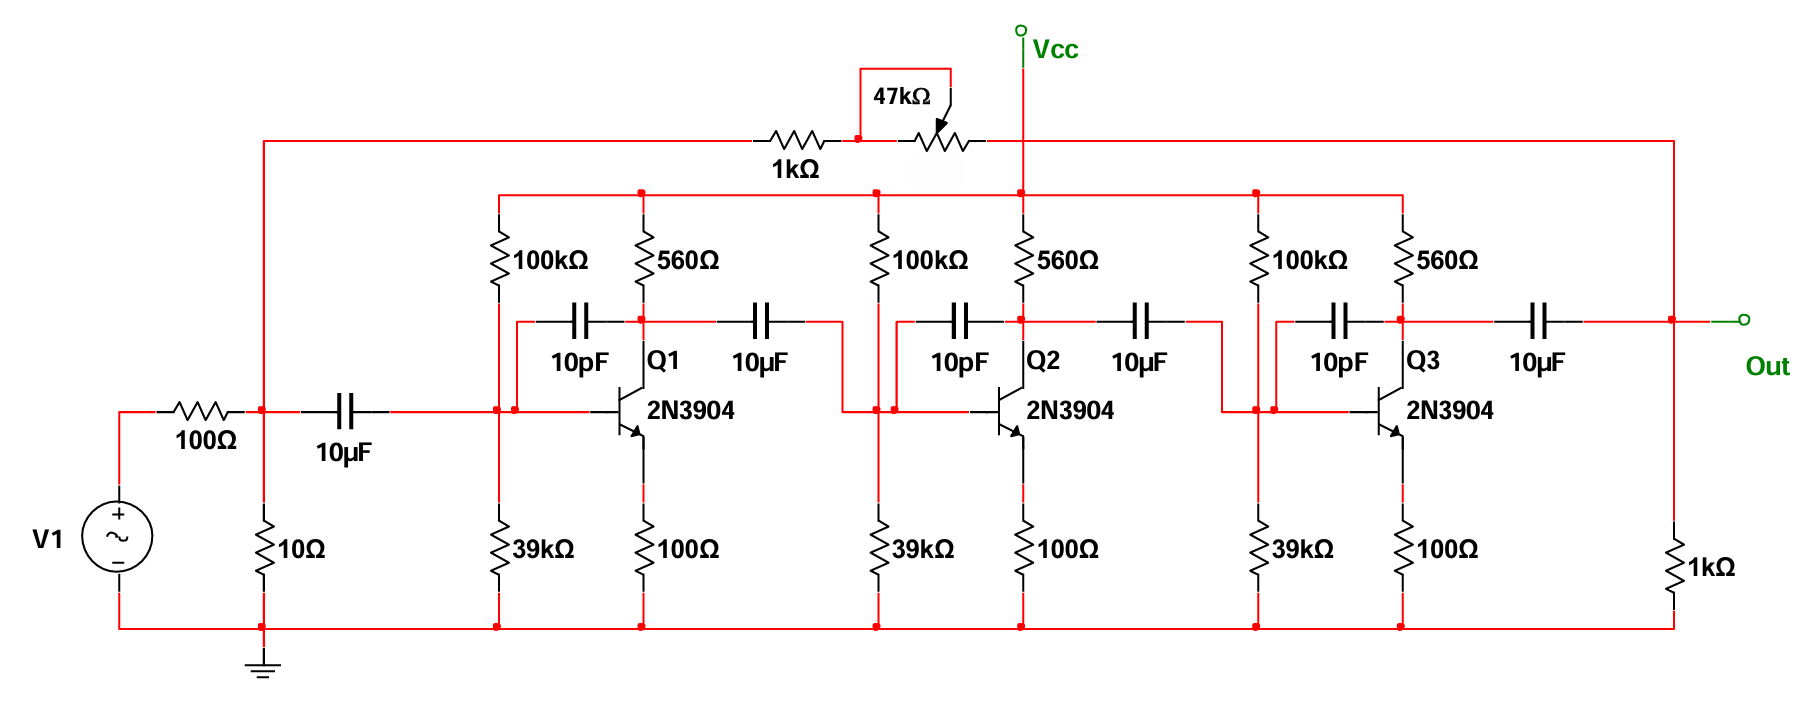
\includegraphics[width=0.47\textwidth]{imagenes/diagrama placa.png}
  \caption{Transistor NPN en configuración de emisor común.}
  \label{fig:etapaemisorcomun}
\end{figure}

\begin{figure}[H]
  \centering
  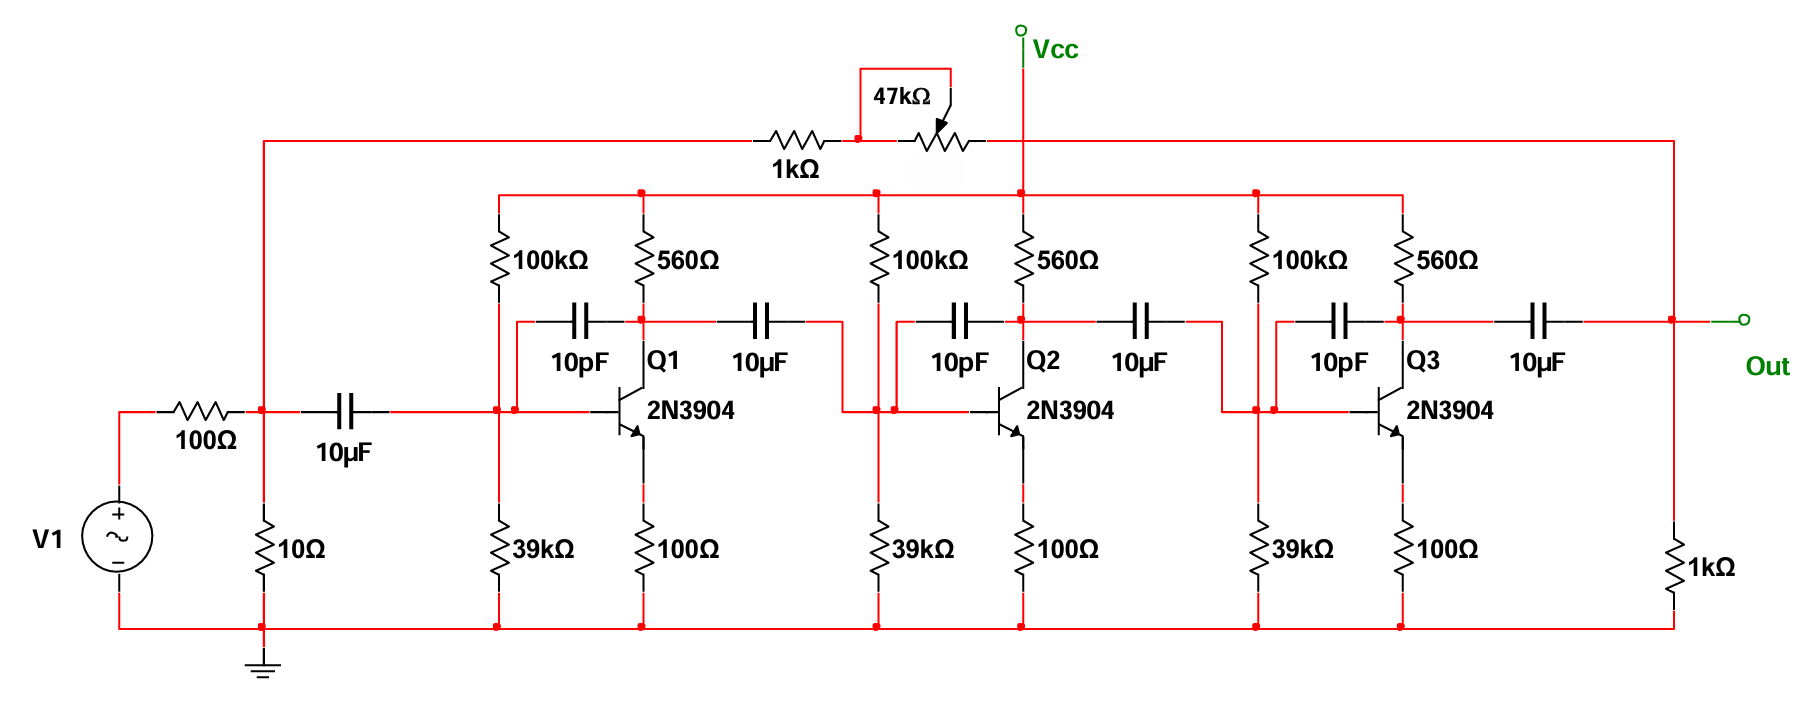
\includegraphics[width=0.47\textwidth]{imagenes/diagrama placa.png}
  \caption{Transistor NPN en configuración de emisor común, según su modelo de pequeña señal.}
  \label{fig:etapaemisorcomunpequeniasenial}
\end{figure}

\subsubsection{Ganancia de Tensión $Av$ de una etapa individual (etapas 1 y 2).}

Del modelo de pequeña señal, y aproximando la corriente del Emisor como $gmV_{\pi}$, se obtiene el siguiente sistema de ecuaciones:

\begin{equation}
\left\{
\begin{aligned}
V_o &= -g_m V_{\pi}R_C \\ 
V_{\pi} &= V_i - V_{R_e} \Longrightarrow V_i = V_{\pi}(gmR_e + 1)\\
\end{aligned}
\right.
\end{equation}

Por lo que la ganancia $Av = \frac{V_o}{V_i}$, considerando el producto $gmR_e >> 1$, será:

\begin{equation}
Av_{1,2} = \frac{-gmR_c}{gmR_e+1} \approx -\frac{R_c}{R_e}
\end{equation}

Para el caso particular de estudio con valores $R_c = 560\Omega$ y $R_e = 100\Omega$, la ganancia de tensión de la etapa individual 1 y 2 es:

\begin{equation}
Av_{1,2} \approx -\frac{560\Omega}{100\Omega} \approx -5,6 \\[1em]
\end{equation}

\subsubsection{Impedancia de entrada $Z_{in}$}\\

\subsubsection{Impedancia de salida $Z_{out}$}\\

\subsubsection{Ganancia de Tensión $Av$ de la última etapa}
La salida de la útlima etapa se ve cargada por un resistor de $1k\Omega$. La ganancia se obtiene de igual manera que las etapas anteriores, pero la carga será el resistor del colector $R_c$ ahora en paralelo con el resistor de $1k\Omega$:

\begin{equation}
Av_3 \approx -\frac{R_c//1k\Omega}{R_e} \approx -3,58
\end{equation}

\subsection{\textbf{Amplificador Multietapa a Lazo Abierto.}}
El circuito a utilizar consta de tres etapas en cascada de transistores BJT NPN idénticas a las analizadas en la sección previa, con una resistencia de $1k\Omega$ conectada como carga a la salida.\\

\subsubsection{Ganancia de Tensión $Av_{LA}$ Multietapa a Lazo Abierto}

En la sección previa se verificó que cada etapa individual presenta una alta impedancia de entrada y una baja impedancia de salida, de modo que puede considerarse que las tres etapas en cascada se acoplan tal que la ganancia total es el producto de las ganancias de cada etapa:\\

\begin{equation}
Av_{LA} \approx Av_1  Av_2  Av_3 \approx (-5,6)(-5,6)(-3,58) \approx -112,26
\end{equation}

\subsubsection{Ganancia de Transimpedancia $Az_{LA}$ Multietapa a Lazo Abierto}

Para el análisis posterior sobre realimentación, resulta de interés convertir la ganancia $Av_{LA}$ en una ganancia de Transimpedancia $Az_{LA} =\frac{V_o}{I_i}$. Esto se logra reescribiendo la tensión de entrada $V_o$ en función de la corriente de entrada $I_i$, obteniendo:

\begin{equation}
Az_{LA} = Av_{LA} . Z{in} = 99.99 = 99
\end{equation}

\subsubsection{Impedancia de entrada del Amplificador Multietapa a Lazo Abierto $Z_{in}$}

La impedancia de entrada será la misma que la de la primer etapa individual:

\begin{equation}
Z_{in} \approx 99
\end{equation}

\subsubsection{Impedancia de salida del Amplificador Multietapa a Lazo Abierto $Z_{out}$}\\

La impedancia de salida será la misma que la de la última etapa individual:

\begin{equation}
Z_{out} \approx 99
\end{equation}

En la \textit{Figura 3} se presenta un diagrama circuital de la placa utilizada:

\begin{figure}[H]
  \centering
  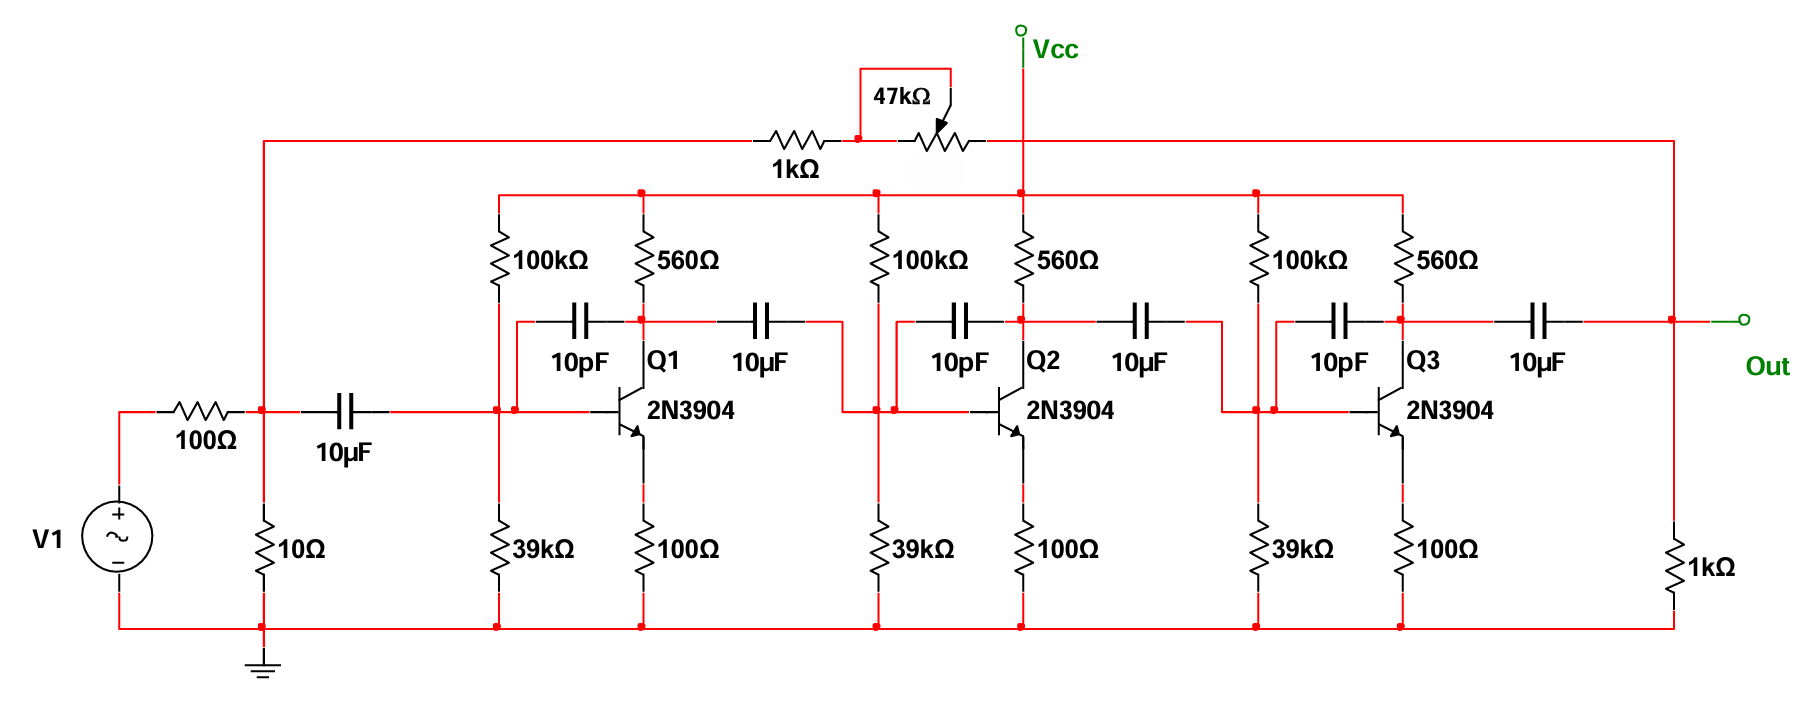
\includegraphics[width=0.47\textwidth]{imagenes/diagrama placa.png}
  \caption{Diagrama circuital de la placa utilizada.}
  \label{fig:diagramaplaca}
\end{figure}

\subsection{\textbf{Amplificador multietapa Realimentado.}}

La realimentación se da por una rama desde la entrada de la primer etapa a la salida de la última, compuesta por un bloque beta que contiene un resistor y un potenciómetro en serie, de manera tal que se pueda variar la resistencia del bloque Beta entre y $1k\Omega$ y $48k\Omega$.\\

\subsubsection{Ganancia de Tensión $Az_{cargado}$}

Para obtener la ganancia final del cirucito realimentado, se precisa conocer primero la ganancia $A_{cargado}$, correspondiente al bloque $A$ cargado con el bloque $\beta$.\\
La topología que presenta es Paralelo-Paralelo, que corresponde a un amplificador de Transimpedancia.\\
Se propone analizar el circuito en bloques. La topología que se ajusta al circuito es la del siguiente diagrama:

\begin{figure}[H]
  \centering
  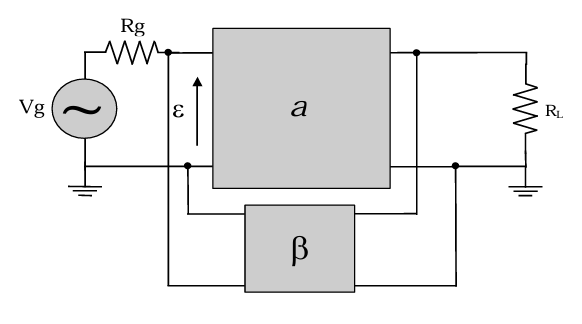
\includegraphics[width=0.47\textwidth]{imagenes/topologia.png}
  \caption{Topología Paralelo-Paralelo correspondiente a un circuito amplificador de Transimpedancia.}
  \label{fig:diagrama_bloques_realimentacion}
\end{figure}

\begin{figure}[H]
  \centering
  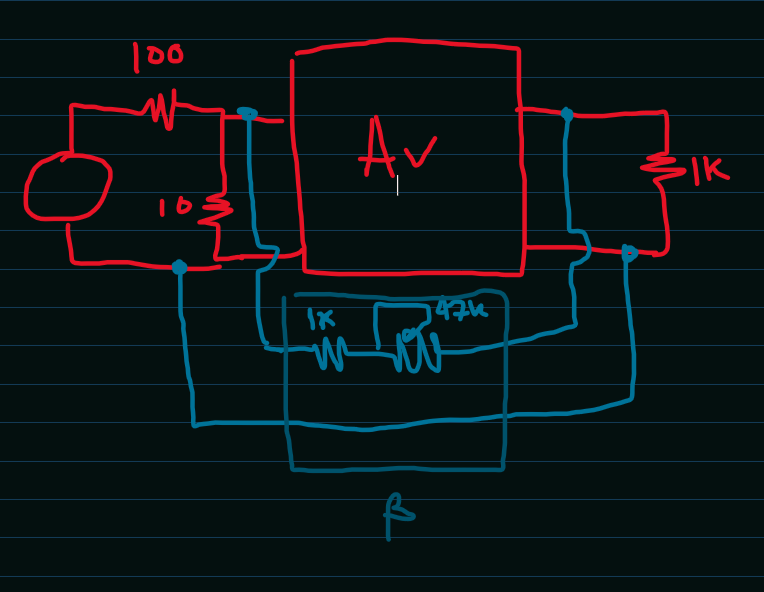
\includegraphics[width=0.47\textwidth]{test1.png}
  \caption{Diagrama en bloques del circuito realimentado.}
  \label{fig:diagrama_bloques_realimentacion}
\end{figure}

Donde el bloque Beta posee los valores de transferencia de transadmitancia $\beta$, admitancia de entrada $y_{i\beta}$ y admitancia de salida $y_{o\beta}$ representados por los parámetros $Y$ listados a continuación:

\begin{equation}
\begin{aligned}
\beta &= y_{12} = \frac{I_1}{U_2} \bigg\rvert_{U_1 = 0} = -\frac{1}{R_f} \\[1em]
y_{i\beta} &= y_{11} = \frac{I_1}{U_1} \bigg\rvert_{U_2 = 0} = \frac{1}{R_f}\\[1em]
y_{o\beta} &= y_{22} = \frac{I_2}{U_2} \bigg\rvert_{U_1 = 0} = \frac{1}{R_f}\\
\end{aligned}
\end{equation}

Con $R_f = 1k\Omega + R_p$ ($R_p$ siendo la resistencia variable del potenciómetro).\\
Calculando para valores extremos de $R_f$:\\

\begin{itemize}
  \item $R_f = 1k\Omega$

    \begin{equation}
    \begin{aligned}
    &\beta = -\frac{1}{1k\Omega} =  -1 mS\\[1em]
    &y_{i\beta} = \frac{1}{1k\Omega} =  1 mS\\[1em]
    &y_{o\beta} = \frac{1}{1k\Omega} = 1 mS\\
    \end{aligned}
    \end{equation}

  \item $R_f = 48k\Omega$
  
  \begin{equation}
    \begin{aligned}
    &\beta = -\frac{1}{48k\Omega} =  -20,83\mu S\\[1em]
    &y_{i\beta} = \frac{1}{48k\Omega} =  20,83\mu S\\[1em]
    &y_{o\beta} = \frac{1}{48k\Omega} = 20,83\mu S\\
    \end{aligned}
    \end{equation}
  
\end{itemize}

Incluyendo $y_{11}^{-1}$ y $y_{22}^{-1}$ dentro del bloque A, se obtiene la ganancia $Av_{cargado}$ del bloque \textit{A} cargado:

\begin{figure}[H]
  \centering
  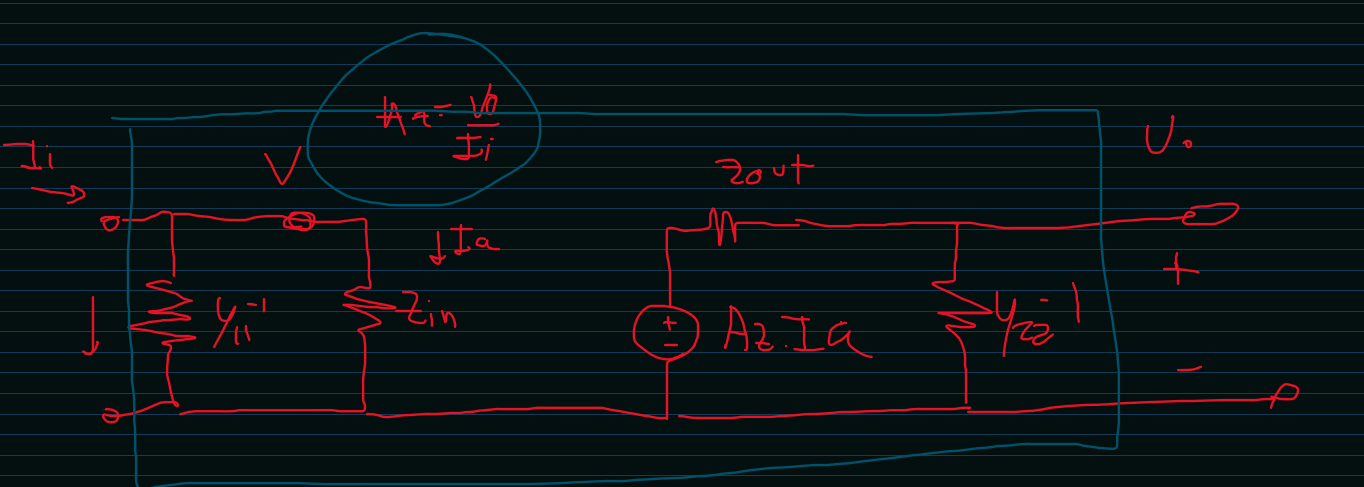
\includegraphics[width=0.47\textwidth]{imagenes/acargado.png}
  \caption{Bloque A cargado.}
  \label{fig:diagrama_bloques_realimentacion}
\end{figure}

La ganancia de transimpedancia $Az_{cargado} = \frac{V_o}{I_i}$ se obtiene planteando el siguiente sistema de ecuaciones:

\begin{equation}
\left\{
\begin{aligned}
V_o &= \frac{Az_{LA} I_a y_{22}^{-1}}{y_{22}^{-1}+Z_{out}} \\ 
I_a &= \frac{I_1}{Z_{in}(y_{11}+Z_{in}^{-1})}\\
\end{aligned}
\right.
\end{equation}

Resulta:

\begin{equation}
Az_{cargado} = \frac{V_o}{I_i} =  \frac{Az_{LA}}{(1+Z_{out}y_{22})(y_{11}Z_{in}+1)}\\[1em]
\end{equation}

\subsubsection{Ganancia de Transimpedancia $Az_r$ del circuito realimentado}

Para obtener la ganancia de Tensión $Av_r$ del circuito realimentado, nos valemos de la siguiente fórmula:

\begin{equation}
Az_r = \frac{Az_{cargado}}{1+\beta Az_{cargado}}
\end{equation}

Donde $Az_{cargado}$ corresponde a la ganancia del bloque $A$ cargado con el bloque $\beta$, mientras que $\beta$ es la transferencia $\frac{I_1}{V_2}$ del bloque de realimentación, ambas obtenidas en la sección anterior.\\
Finalmente, se obtiene:

\begin{equation}
Az_r = \frac{99}{1+1mS 99} = 99\\
\end{equation}

\subsubsection{Impedancia de entrada $Zin_{r}$ del circuito realimentado}

La impedancia de entrada disminuye al realimentar, por un factor de $1+\beta Az_{cargado}$:

\begin{equation}
Zin_r = \frac{Z_i}{1+\beta Az_{cargado}} = 99\\
\end{equation}

\subsubsection{Ganancia de Tensión $Av_r$ del circuito realimentado}

En el desarrollo del laboratorio se pretende medir ganancia de tensión del circuito completo. Es por ello que es preferible transformar la ganancia de transimpedancia $Az_r$ a una ganancia de tensión $Av_r = \frac{V_o}{V_2}$:

\begin{figure}[H]
  \centering
  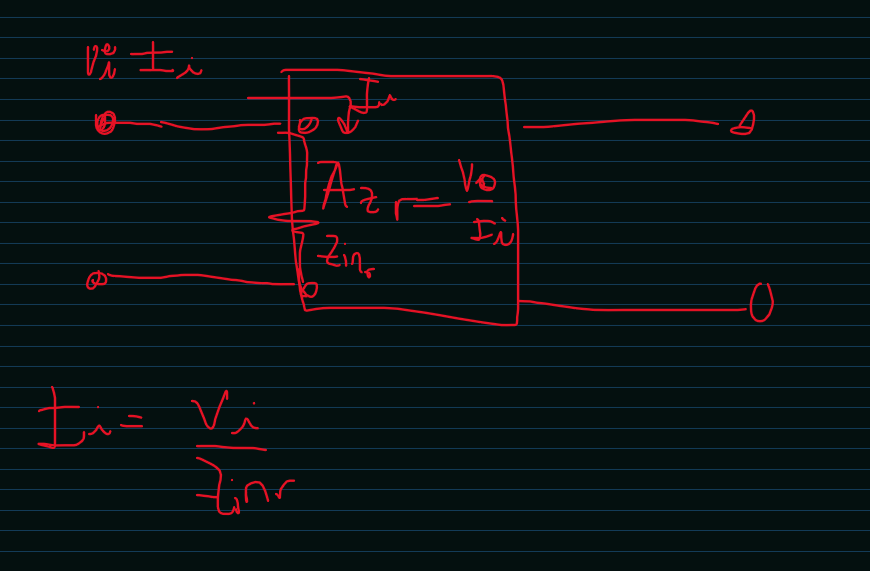
\includegraphics[width=0.47\textwidth]{imagenes/transf.png}
  \caption{Diagrama del bloque cargado expresado como amplificador de transimpedancia. Se planteó $I_i$ en funcion de $V_i$}
  \label{fig:diagrama_bloques_realimentacion}
\end{figure}

\begin{equation}
I_i = \frac{V_i}{Zin_r}
\end{equation}

Reemplazando en $Az_r = \frac{V_o}{I_o}$:

\begin{equation}
 Az_r = \frac{V_o}{V_i} Zin_r = Av_rZin_r \\
\end{equation}

\begin{equation}
\therefore Av_r = \frac{Az_r}{Zin_r} = 99
\end{equation}

\subsection{Valores extremos}
Como se observa, la resistencia $R_f$ de la rama de realimentación está compuesta por un potenciómetro, que permite fijar en la rama un valor de resistencia entre $1k\Omega$ y $48k\Omega$.\\
A continuación se presentan en forma de tabla los valores numéricos de los parámetros obtenidos en esta sección, para los casos extremos de realimentación:


\begin{table}[h]
\begin{center}
\begin{tabular}{|c||c|c|c|}
\hline
$R_f$ & Ecuación & $1k\Omega$ & $48k\Omega$\\
\hline
$\beta$ & (9) & -$1 mS$ & $-20,83\mu S$\\
\hline
$y_{i\beta}$ & (9) & $1 mS$ & $20,83\mu S$\\
\hline
$y_{o\beta}$ & (9) & $1 mS$ & $20,83\mu S$\\
\hline
$Az_{cargado}$ & (13) & $48k\Omega$ (máx.) & 8.5kHz\\
\hline
$Zin_r$ & (16) & $1 mS$ & $20,83\mu S$\\
\hline
$Az_r$ & 1 & $48k\Omega$ (máx.) & 8.5kHz\\
\hline
$Av_r$ & 1 & $48k\Omega$ (máx.) & 8.5kHz\\
\hline
\end{tabular}
\end{center}
\caption{Parámetros numéricos del amplificador, para casos extremos de $R_f$.}
\label{tab:parametros}
\end{table}



\section{Desarrollo experimental}
Se describirán a continuación las mediciones hechas y los resultados obtenidos.\\
La placa consiste en un amplificador multietapa realimentado, como el estudiado en la sección del Marco Teórico.\\
Se propuso entonces medir dos factores: la ganancia de tensión realimentada; y el ancho de banda, ambos para los valores extremos de las resistencias de realimentación del bloque beta.

\subsection{Conexiones y consideraciones para la medición}

\begin{itemize}
  \item Se administró una tensión continua de polarización de $12V$,
  \item Se conectó un generador de funciones a la entrada, entre los terminales 'E' y tierra. La función suministrada será siempre una onda senoidal de $400mV Vpp$,
  \item Se conectó un osciloscopio a la entrada y a la salida, quedando representadas siempre la entrada en color amarillo, y la salida en azul.
\end{itemize}

\begin{figure}[H]
  \centering
  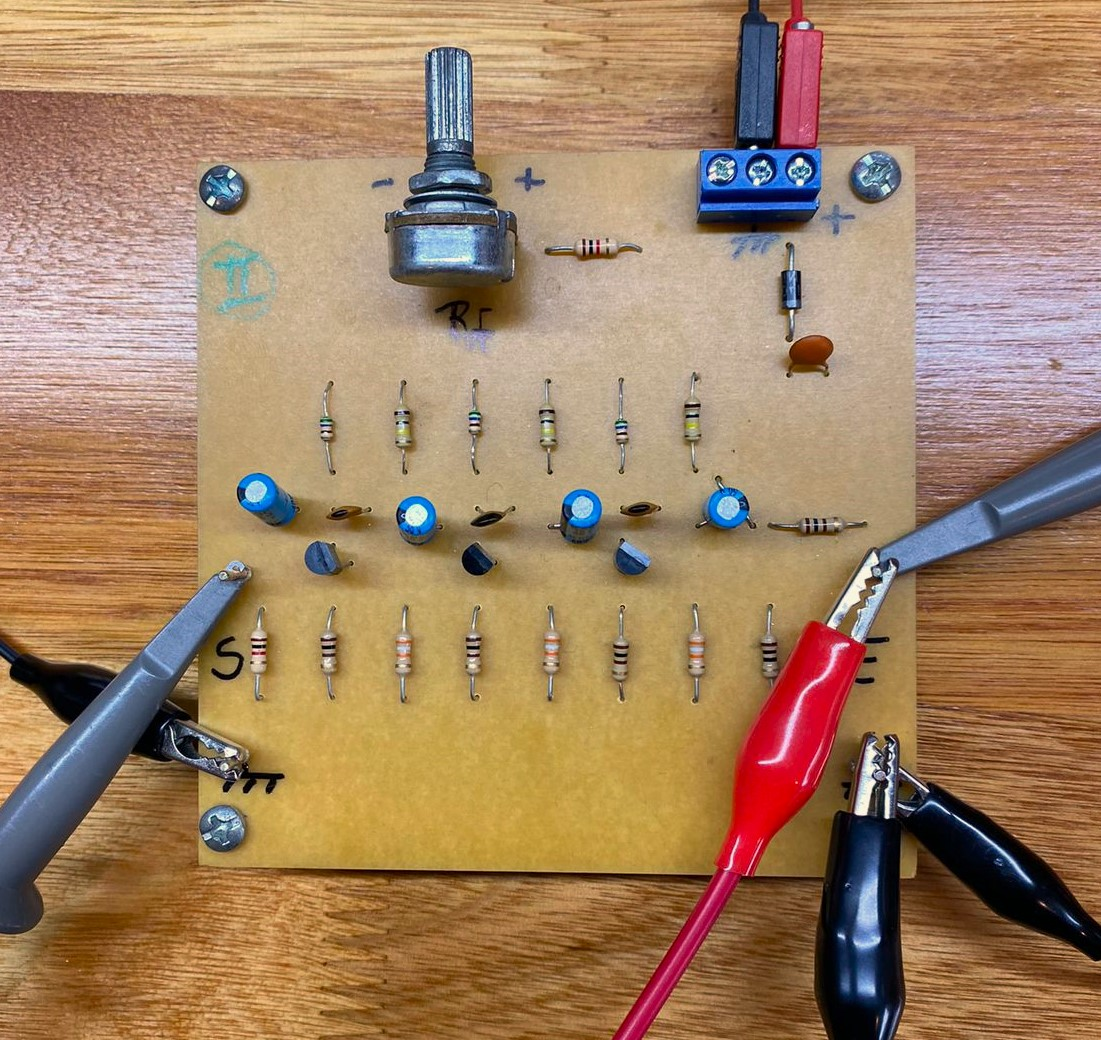
\includegraphics[width=0.47\textwidth]{imagenes/placa conectada.jpg}
  \caption{Conexión final de los instrumentos a la placa}
  \label{fig:placaconectada}
\end{figure}

\subsection{Ganancia de Tensión Realimentada $Av_r$}

Se pocedió entonces a la medición de la Ganancia de Tensión con el circuito realimentado, inyectando una señal senoidal de $400mV Vpp$ y frecuencia $khz$.
La frecuencia elegida se consideró lo suficientemente baja como para no verse afectada por el polo dominante del circuito.\\

\subsubsection{Potenciómetro en mínimo}

Primeramente, se dispuso el potenciómetro en mínimo ($0\Omega$), quedando el bloque Beta compuesto solo por la resistencia de $1k\Omega$.
Para la entrada de $400mV Vpp$, se midió una salida de $99$:

\begin{figure}[H]
  \centering
  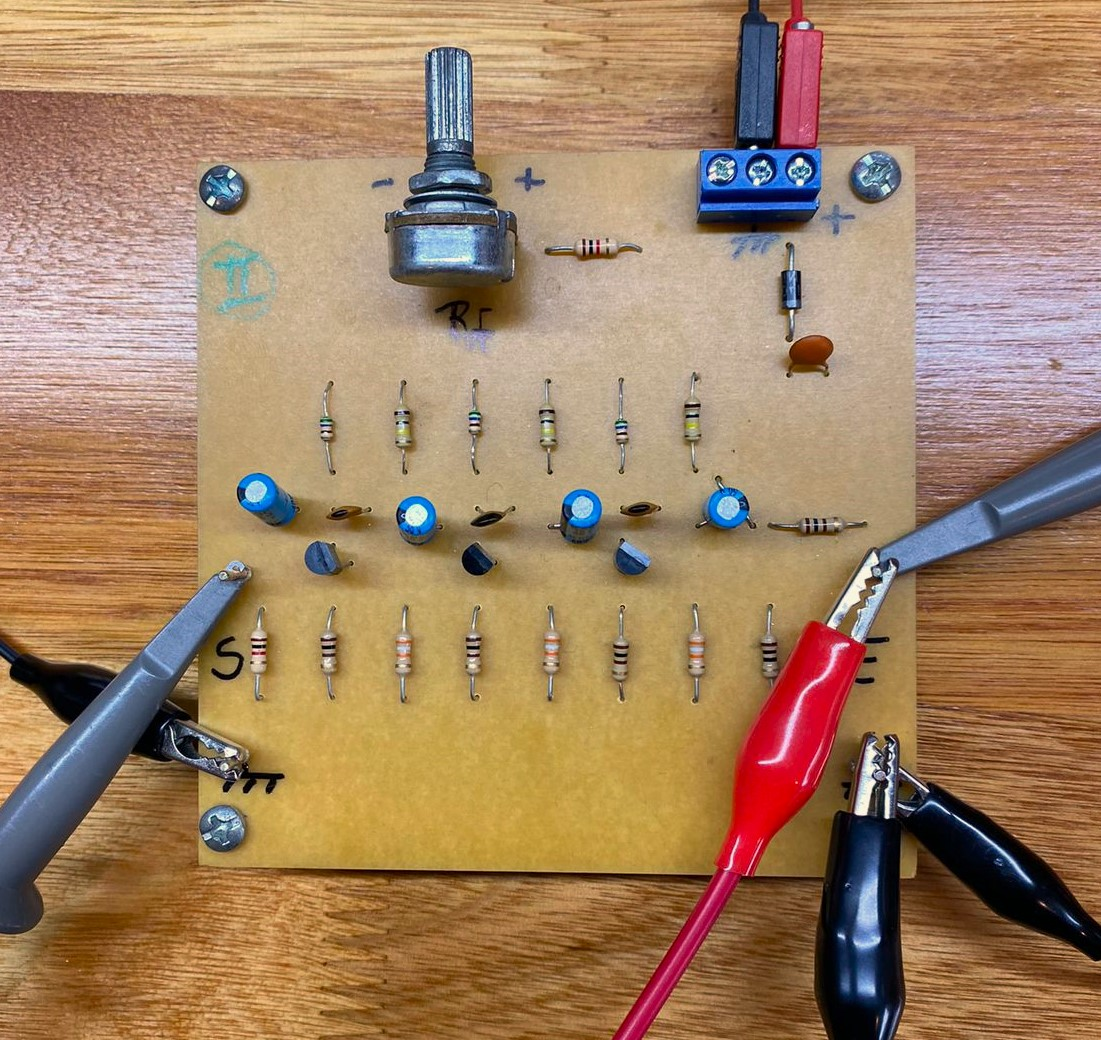
\includegraphics[width=0.47\textwidth]{imagenes/placa conectada.jpg}
  \caption{La señal de salida (azul) es $99$ veces mayor que la entrada, para una realimentación de $1k\Omega$}
  \label{fig:osciloscopio_ganancia_pote_max}
\end{figure}

\subsubsection{Potenciómetro en máximo}

A continuación, se subió el potenciómetro a su valor máximo ($47k\Omega$), quedando el bloque Beta como una resistencia de $48k\Omega$.
Para la entrada de $400mV Vpp$, se midió una salida de $99$:

\begin{figure}[H]
  \centering
  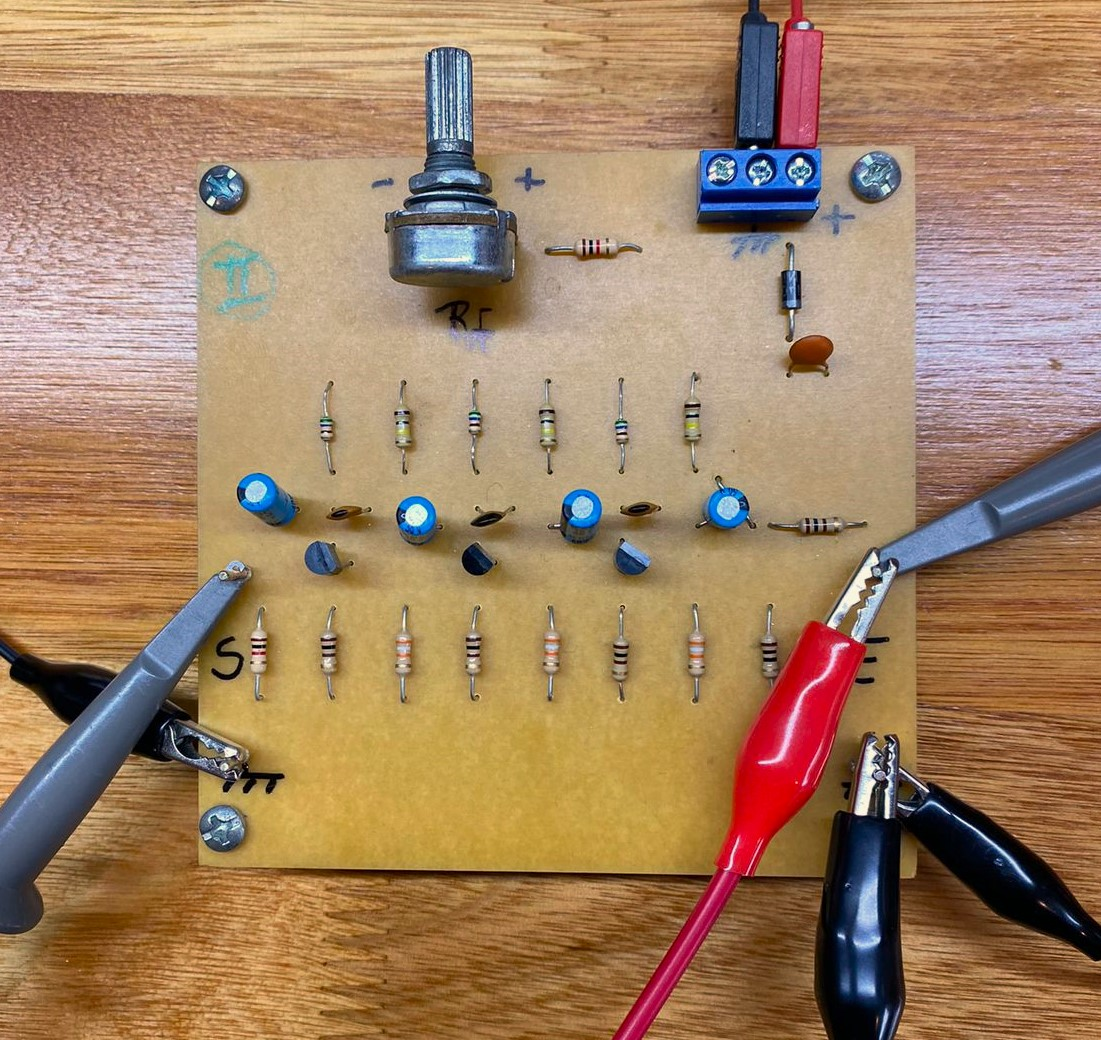
\includegraphics[width=0.47\textwidth]{imagenes/placa conectada.jpg}
  \caption{La señal de salida (azul) es $99$ veces mayor que la entrada, para una realimentación de $47k\Omega$}
  \label{fig:osciloscopio_ganancia_pote_max}
\end{figure}

\subsection{Ancho de banda}

Para estudiar el ancho de banda se realizó un barrido de frecuencia desde $10k\Omega$ hasta medir en la salida una atenuación de $3dB$.\\

\subsubsection{Potenciómetro en mínimo}
Para el potenciómetro en mínimo se obtuvo previamente una salida de $99$, por lo que su polo estará ubicado donde se produzca una atenuación de $3dB$, es decir, cuando su valor de salida sea $\frac{x}{\sqrt{2}} = $

\begin{figure}[H]
  \centering
  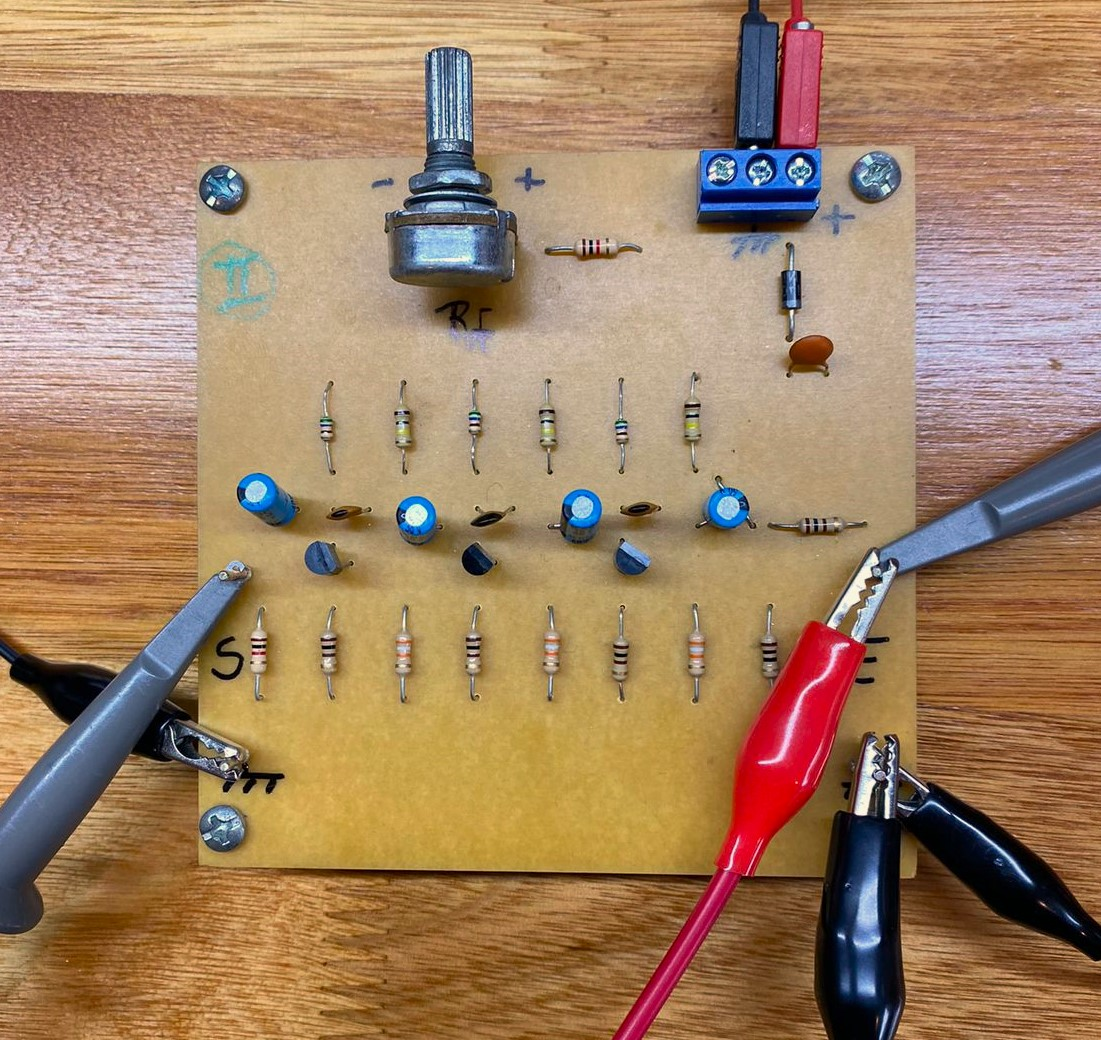
\includegraphics[width=0.47\textwidth]{imagenes/placa conectada.jpg}
  \caption{Se midió una atenuación de $3dB$ a una frecuencia de $99Hz$}
  \label{fig:osciloscopio_freq_pote_min}
\end{figure}

\subsubsection{Potenciómetro en máximo}
Para el potenciómetro en máximo se obtuvo previamente una salida de $99$, por lo que su polo estará ubicado donde se produzca una atenuación de $3dB$, es decir, cuando su valor de salida sea $\frac{x}{\sqrt{2}} = $

\begin{figure}[H]
  \centering
  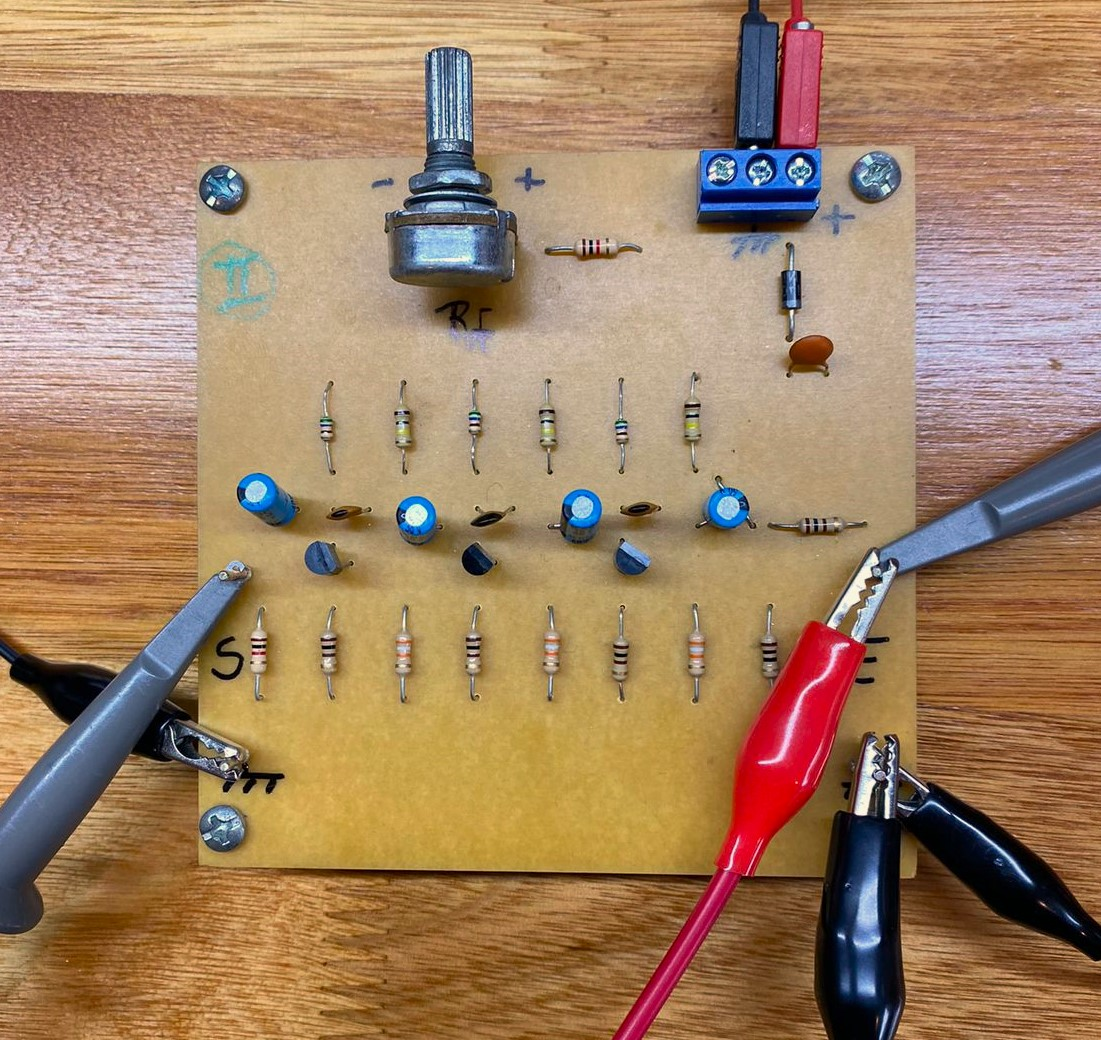
\includegraphics[width=0.47\textwidth]{imagenes/placa conectada.jpg}
  \caption{Se midió una atenuación de $3dB$ a una frecuencia de $99Hz$}
  \label{fig:osciloscopio_freq_pote_max}
\end{figure}

A continuación se 

\begin{table}[h]
\begin{center}
\begin{tabular}{|c||c|}
\hline
Resistencia Bloque Beta & Frecuencia de corte\\
\hline
$1k\Omega$ (mín.) & 27kHz\\
\hline
$48k\Omega$ (máx.) & 8.5kHz\\
\hline
\end{tabular}
\end{center}
\caption{Mediciones de compensación}
\label{tab:simple}
\end{table}

\section{Conclusiones}

Los experimentos realizados permitieron verificar el comportamiento teórico de los circuitos integrador y derivador operacionales. Se comprobó que ambos circuitos tienen un rango de operación adecuado, determinado por la ubicación de sus polos. En el caso del integrador, se obtuvo la salida esperada a frecuencias altas, mientras que para el derivador, a frecuencias bajas. El amplificador de instrumentación demostró la capacidad de compensar sus polos, y a su vez sirvió para mostrar un rechazo al modo común.\\
Todas las mediciones y pruebas fueron las esperadas según calculos teóricos previos y se condicen con lo visto en el \textit{Marco Teórico}.
 

\addtolength{\textheight}{-12cm}   % This command serves to balance the column lengths
                                  % on the last page of the document manually. It shortens
                                  % the textheight of the last page by a suitable amount.
                                  % This command does not take effect until the next page
                                  % so it should come on the page before the last. Make
                                  % sure that you do not shorten the textheight too much.

%%%%%%%%%%%%%%%%%%%%%%%%%%%%%%%%%%%%%%%%%%%%%%%%%%%%%%%%%%%%%%%%%%%%%%%%%%%%%%%%



%%%%%%%%%%%%%%%%%%%%%%%%%%%%%%%%%%%%%%%%%%%%%%%%%%%%%%%%%%%%%%%%%%%%%%%%%%%%%%%%



%%%%%%%%%%%%%%%%%%%%%%%%%%%%%%%%%%%%%%%%%%%%%%%%%%%%%%%%%%%%%%%%%%%%%%%%%%%%%%%%



%\section*{ACKNOWLEDGMENT}

%The preferred spelling of the word Òacknowledgment\'o in America is without an Òe\'o after the Òg\'o. Avoid the stilted expression, ÒOne of us (R. B. G.) thanks . . .\'o  Instead, try ÒR. B. G. thanks\'o. Put sponsor acknowledgments in the unnumbered footnote on the first page.



%%%%%%%%%%%%%%%%%%%%%%%%%%%%%%%%%%%%%%%%%%%%%%%%%%%%%%%%%%%%%%%%%%%%%%%%%%%%%%%%


\begin{thebibliography}{99}

\bibitem{c1} J. Millman and A. Grabel, ``Microelectrónica,” McGraw-Hill, New York, 6ta edición, 1993.
\bibitem{c2} P. R. Gray and R. G. Meyer, ``Analysis and Design of Analog Integrated Circuits,” John Wiley & Sons, New York, 4th edition, 2001



\end{thebibliography}




\end{document}
